\subsection{Channel-wise and Spatial Feature Modulation Network (CSFM\cite{CSFM})}

CSFM exploit features reuse with dense connections, ease the training with skip and dense connections as well as avoid the flow of low-level features inside the network and focus on high-frequency information  and on particular spatial position using channel-wise and spatial-wise attention mechanisms.

\subsubsection{Architecture}
\begin{figure}
    \centering
    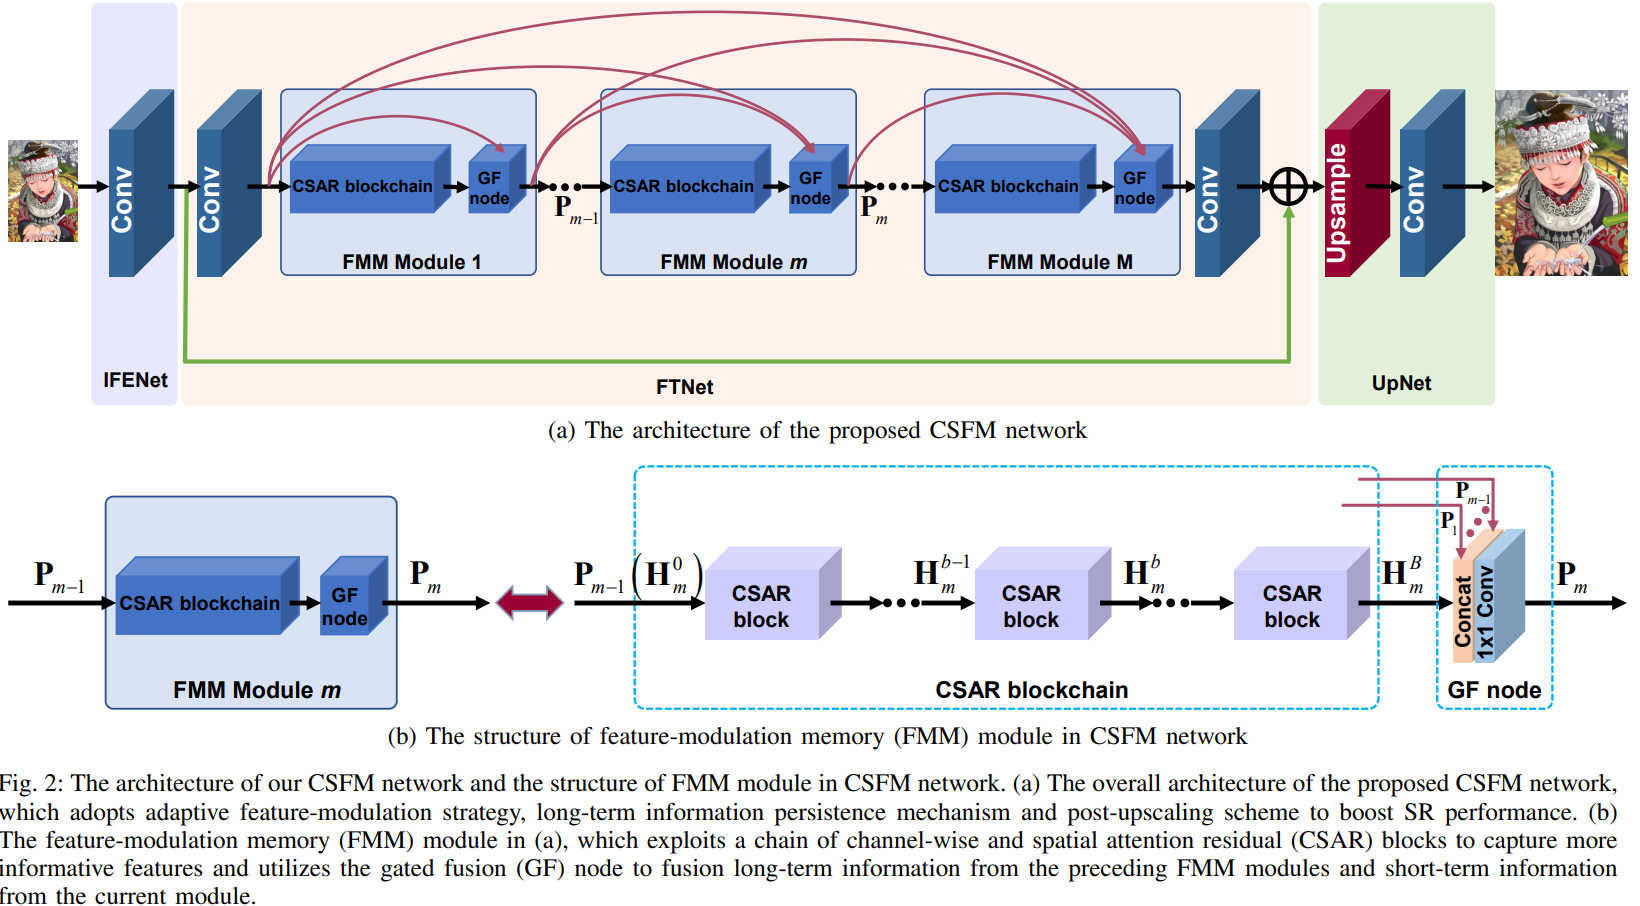
\includegraphics[width=\textwidth, keepaspectratio]{csfm-model.png}
    \caption{CSFM architecture.}\label{csfm:architecture}
\end{figure}

\begin{figure}
    \centering
    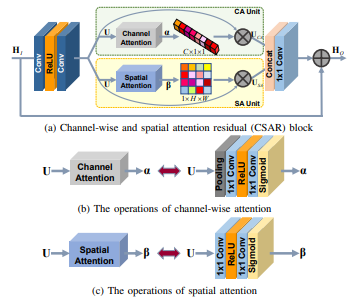
\includegraphics[width=0.6\textwidth, keepaspectratio]{csfm-csar-module.png}
    \caption{CSAR block.}\label{csfm:csar}
\end{figure}

\paragraph{Feature-Modulation Memory}
\textbf{CSFM} contains stacked \textbf{feature-modulation memory} (\textit{FMM}) which contains a \textbf{CSAR blockchain} and a \textbf{GF node}.

Since the \textbf{gated-function node} (\textit{GF node}) processes not only the features received by the \textit{CSAR blockchain} but also the ones from the output of all previous FMMs, it is preserving long-term features information.

These information flow from one FMM to another but also in the network from shallow levels to deeper ones thanks to the dense connection, this ease the training but also allow to create features at multiple levels.

The \textit{CSAR blockchain} is a sequence of \textbf{Channel and spatial attention residual block} (\textit{CSAR}[\Cref{csfm:csar}]).

\subparagraph{Channel and spatial attention residual block} \textbf{CSAR} is a residual block where there is an identity skip connection that flow low-frequency information, ease the training and preserve shotr-term information and a residual path where a \textbf{channel attention} and \textbf{spatial attention} mechanisms are used for extracting high-frequency information feature-wise and spatial-wise.

\subparagraph{CA and SA}
The  \textbf{channel attention}(\textit{CA}) and \textbf{spatial attention}(\textit{SA}) are both used for creating a mask in order to improve the expressive power of the network.

The \textit{CA} extract a channel-wise statistics from the residual processed in \textit{CSAR} using global averaging pooling and processing non-linear features with a sigmoid.

The \textit{SA} extract a spatial-wise statistics simply expanding the channel with the convolution, extracting non-linear features, reducing the channel to the original number and then computing the mask with the same spatial dimension as the input.

\subsubsection{Results}

\paragraph{Ablation studies}
The [\Cref{csfm:ablationstudies}] have proved the efficacy of the CA, SA (since they are able to increase high-frequency information) and GF (since it's able to process long-term information along the network).
\begin{figure}[H]
    \begin{subfigure}{\textwidth}
        \centering
        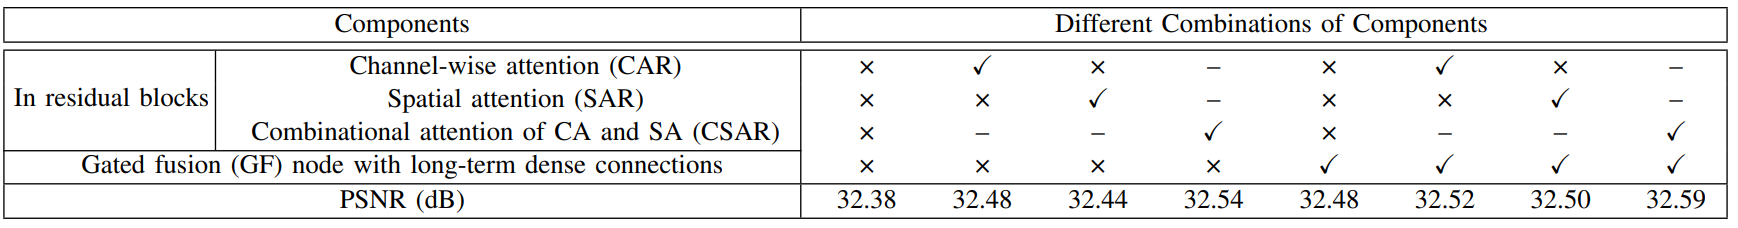
\includegraphics[width=\textwidth, keepaspectratio]{csfm-ablation-studies.png}
    \end{subfigure}
    \begin{subfigure}{\textwidth}
        \centering
        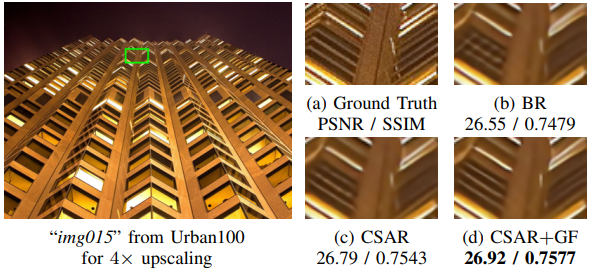
\includegraphics[width=\textwidth, keepaspectratio]{csfm-ablation-studies-visual.png}    
        \caption{Results using BR (simple residual block), CSAR(CA and SA), CSAR and GF}
    \end{subfigure}    
    \caption{Ablation studies for CSFM.}\label{csfm:ablationstudies}
\end{figure}

\paragraph{Analysis of the GF node}
The [\Cref{csfm:gfstudy}] highlights that long-term information are more important than short-term information (the ones coming from the CSAR blockchain) therefore adding GF is important.
\begin{figure}[H]
    \centering
    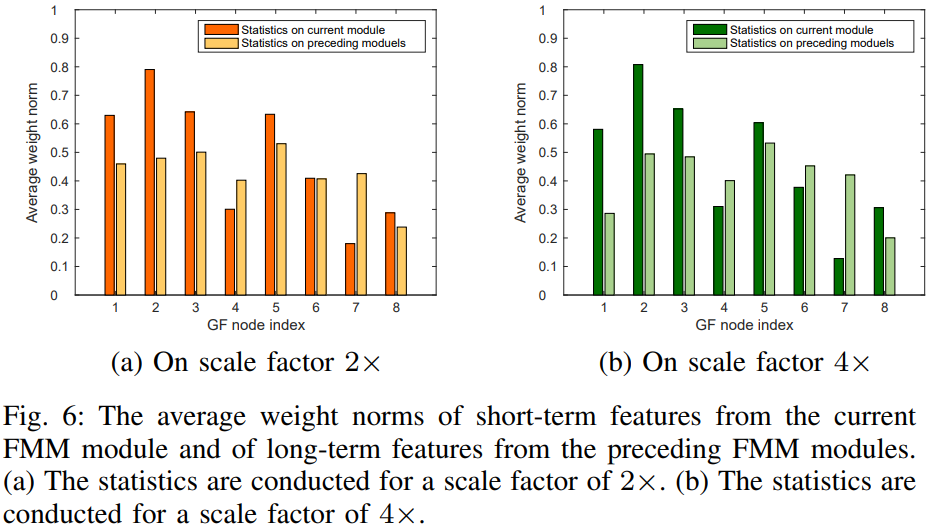
\includegraphics[width=\textwidth, keepaspectratio]{csfm-gf-analysis.png}
    \caption{Normalized weight norms in eight GF nodes of eight FMM
    modules for two scale factors of 2× and 4×.}\label{csfm:gfstudy}
\end{figure}

\paragraph{Number of FMM and CSAR blocks and total amount of parameters}
Increasing B and M allow to have a deeper network hence better performance with low cost in number of parameters.

\begin{figure}[H]
    \centering
    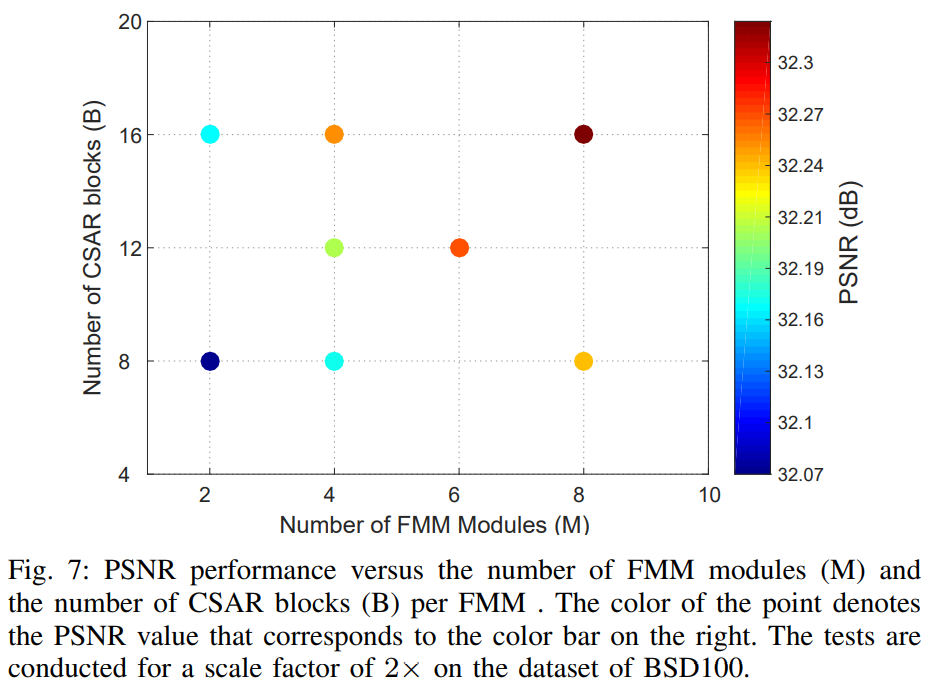
\includegraphics[width=\textwidth,keepaspectratio]{csfm-fmmmodules-csarblocks-psnr.png}
    \caption{Study done on the number of FMM and CSAR blocks.}
\end{figure}
\begin{figure}[H]
    \centering
    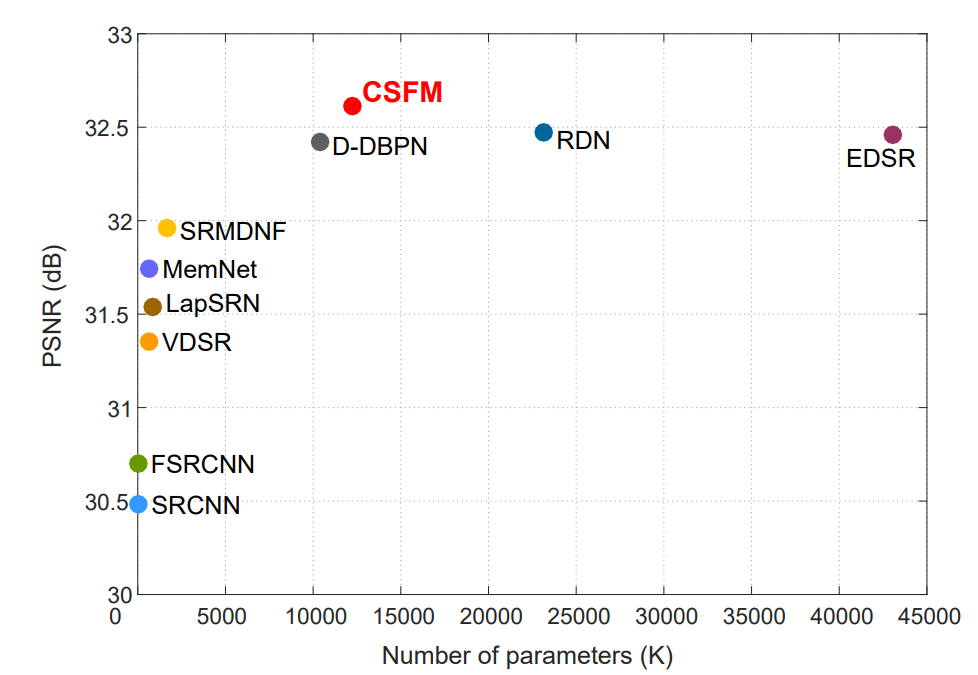
\includegraphics[width=\textwidth, keepaspectratio]{csfm-paramters.png}
    \caption{Number of parameters of CSFM with FMM=8 and CSAR=16}
\end{figure}
\paragraph{Quantitative and qualitative results}
CSFM outperforms all state-of-art-networks.

\begin{figure}[H]
    \centering
    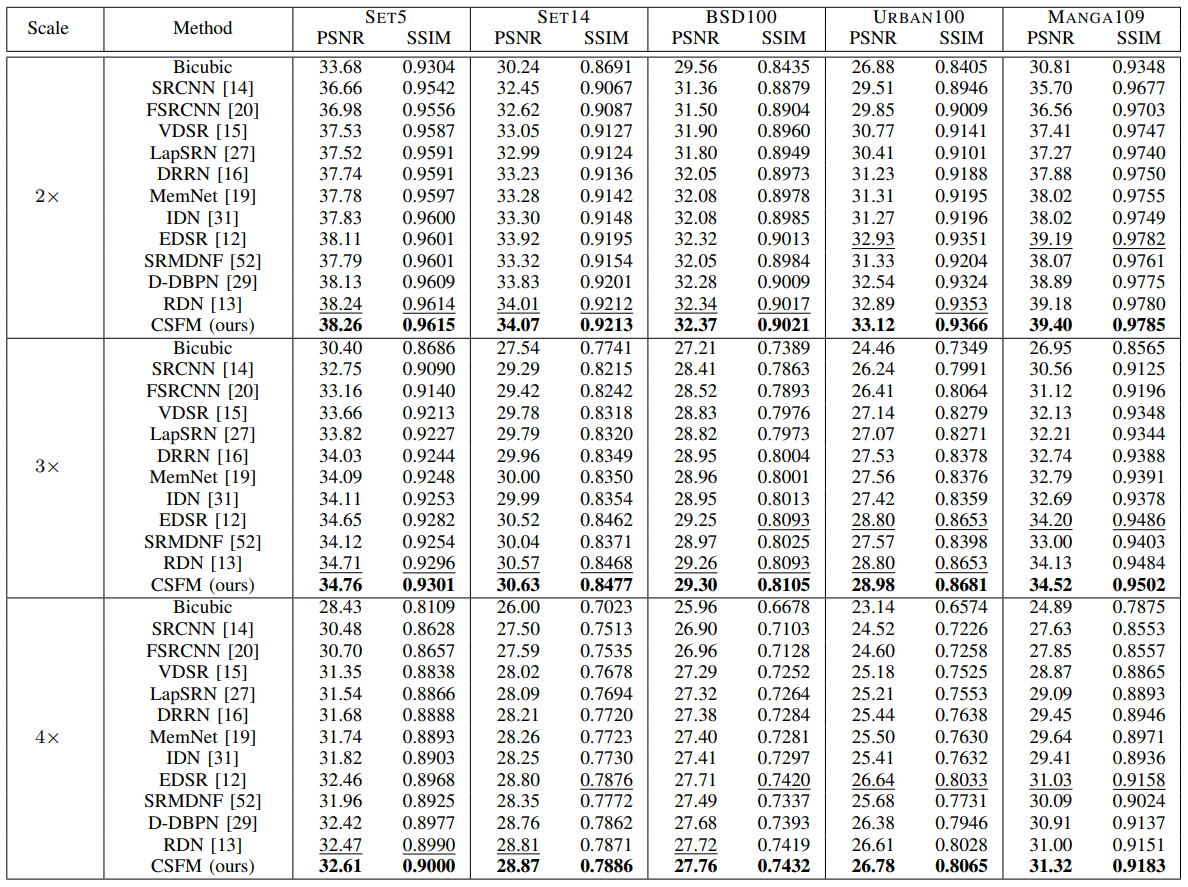
\includegraphics[width=\textwidth, keepaspectratio]{csfm-quantitative.png}
    \caption{Quantitative result of CSFM (FMM=8 and CSAR=16).}
\end{figure}

\begin{figure}[H]
    \centering
    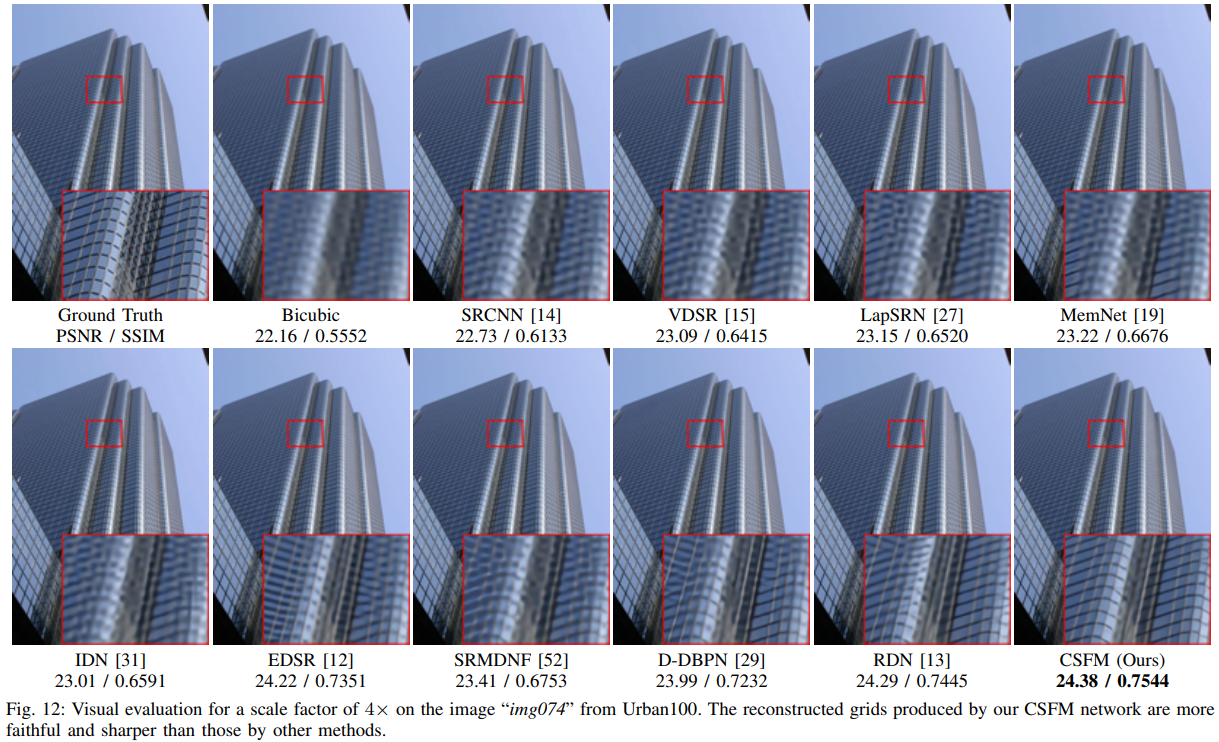
\includegraphics[width=\textwidth, keepaspectratio]{csfm-qualitative.png}
    \caption{Qualitative result of CSFM (FMM=8 and CSAR=16).}
\end{figure}